% -*- latex -*-
\label{chap:kbd}

The PS/2 keyboard interface, designated ‘KBD’, is physically located
on the VDU board (described in~\cfp{chap:hard-vdu}). Since it is
technically a separate interface and originally designed to be built
independently, it is discussed here. Much of the discussion below is based on
\begin{center}
\url{http://www.computer-engineering.org/ps2protocol/} and

\url{http://www.quadibloc.com/comp/scan.htm}.
\end{center}

\section{Design}

\section{Theory of Operation}

\subsection{Physical Interface}

PS/2 keyboard and mice share the same pin-out, in the vast majority connecting
to the host via a 6-pin mini DIN plug. Some devices provide a single socket and
allow a mouse and keyboard to be connected via a short splitter cable which
redirects mouse signals from their (mostly non-standard) locations on the
host's socket to the standard PS/2 interface locations.

Electrically, the PS/2 keyboard interface works on two open drain lines. Each
is pulled to 5V via an appropriate resistor which must be present on the host
side but may be present on the device side too.

The clock line control the timing of data flow. The clock is always generated
by the keyboard or mouse device to ensure that its speed limits are
respected. The frequency of the clock is 10–16.7 kHz (100–60~μs periods). When
both ends of the interface are idle, the clock line is released and allowed to
be pulled up by the resistor (or resistors).

The data line transfers data from one end to the other. When reading from the
device, data is clocked by the host on the falling edge of the clock. When
writing to the device, the device clocks data on the rising edge of the clock.

It is recommended that data is sampled by the host at the middle of the clock
pulse to allow it to settle. This may involve a delay of 30–50~μs.

\begin{figure*}
  \centering
  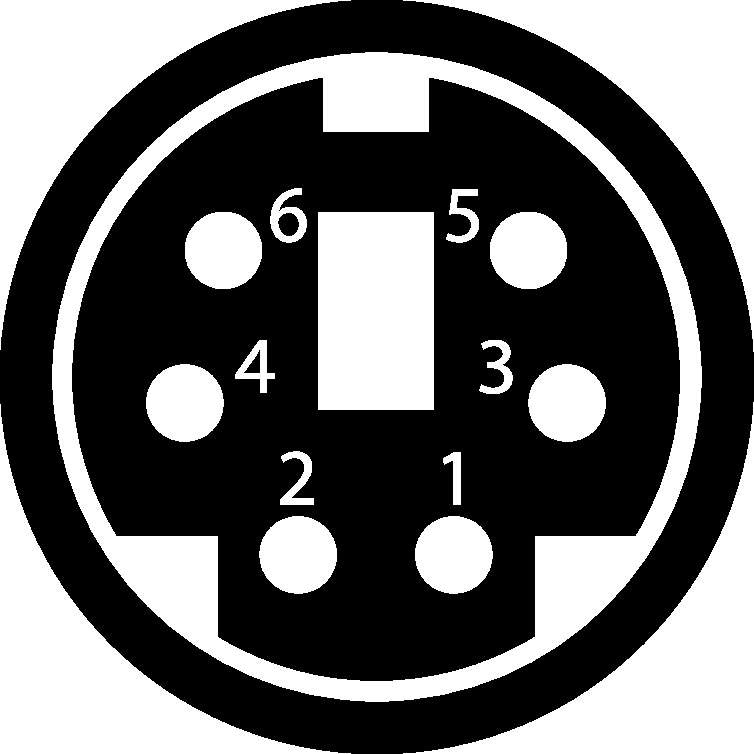
\includegraphics[width=2cm]{figs/MiniDIN-6_Socket_Pinout.pdf}
  \vspace{1em}\par

  \zebra
  \begin{tabular}{clll}
    Pin & Keyboard Port & Mouse Port & Keyboard/Mouse Port \\
    \hline
    1 & Keyboard Data & Mouse Data    & Keyboard Data \\
    2 & Not Connected & Not Connected & Mouse Data \\
    3 & Ground        & Ground        & Ground \\
    4 & +5V DC, 275~mA & +5V DC, 275~mA & +5V DC, 550~mA \\
    5 & Keyboard Clock & Mouse Clock    & Keyboard Clock \\
    6 & Not Connected & Not Connected & Mouse Clock \\
    \hline
  \end{tabular}
  \caption[PS/2 Connector Pin-Out]{\label{fig:kbd-ps2-pinout}PS/2 Connector
    pin-out. This is a view of the PS/2 socket (female connector on mainboards)
    from the front.}
\end{figure*}

\subsection{Communications Protocol}

Both keyboards and mice use the same protocol to exchange data with the
host. Host-to-device and device-to-host directions differ in a number of ways.

\subsubsection{Receiving from the Device}

A timing diagram of a single byte recepction from a device is shown
in~\fcf{fig:kbd-kbd-to-host}. The device only transmits bytes if the clock line
has been consistently high for at least 50~μs. If the clock line is low, the
host is inhibiting reception of new data. Keyboards typically buffer 16 bytes
of data in this case. Mice usually discard data packets.

If the device is clear to transmit, it signals the beginning with the falling
edge of the clock line, and strobes the clock line a total of eleven times:

\begin{description}
\li{Clock 1}: the data line is driven low by the receiver to signal the
beginning of the transmission. This works as a serial start bit.  \li{Clocks
  2–9}: eight data bits are transmitted, least significant bit first.
\li{Clock 10}: an odd parity bit. This bit is clear (\bin{0}) if the number of
set bits in clocks 2–9 (the transmitted byte) is odd. Otherwise, it is set.
\li{Clock 11}: a stop bit, which is always \bin{1}.
\end{description}

The host may stop the device from transmitting at any time by driving the clock
line down for at least 100~μs. Packets may still be transmitted until this
condition is met. If the condition is met during a packet transmission, the
device aborts it, and will restart the entire transmission once the clock line
is released by the host. If this is part of a multi-byte sequence, it will be
restarted from its first byte.

\begin{figure*}
\centering
\begin{tikztimingtable}
  Clock           & 5H 11{CL CH} 5H \\
  Data            & 4H 4L 4D{D0} 4D{D1} 4D{D2} 4D{D3} 4D{D4} 4D{D5} 4D{D6} 4D{D7} 4D{P} 10H \\
\end{tikztimingtable}
\caption[Keyboard/Mouse to Host Communication]{\label{fig:kbd-kbd-to-host}
  Timing of Device (keyboard or mouse) to Host communication. Every byte sent
  includes a start bit (always low), eight bits of data (least significant bit
  first), an odd parity bit, and a stop bit (always high). Eleven clock pulses
  are sent in all. The host clocks data in on the falling edge of the clock
  signal.}
\end{figure*}



\subsubsection{Transmitting to the Device}

A timing diagram of a single byte recepction from the host to a device is shown
in~\fcf{fig:kbd-host-to-kbd}. A host-to-device packet consists of 12 bits. Data
is set while the clock line is low and is read by the device while the clock
is high. The bits sent are as follows:

\begin{description}
\li{Clock 1}: a start bit, always \bin{0}.
\li{Clocks 2–9}: eight data bits are transmitted, least significant bit first.
\li{Clock 10}: an odd parity bit. This bit is clear (\bin{0}) if the number of
set bits in clocks 2–9 (the transmitted byte) is odd. Otherwise, it is set.
\li{Clock 11}: a stop bit, which is always \bin{1}.
\li{Clock 12}: an acknowledge bit, {\em transmitted by the device to the host}.
\end{description}

To transmit a byte to the device, the following sequence of actions must be
performed:

\begin{enumerate}
\item Drive the clock line low for at least 100~μs. This inhibits data
transmission from the device.
\item Drive the data line low. This is the start bit of the transmission.
\item Release the clock line. This signals the device that a host transmission
  is taking place. 
\item Wait for the device to drive the clock line low.
\item Set the data line to the first bit of the byte to send.
\item Wait for the device to release the clock line.
\item Repeat the last three steps to send each bit of the byte and the parity bit.
\item Release the data line.
\item Wait for the device to drive data low.
\item Wait for the device to drive clock low. This is the acknowledge bit from the device.
\item Wait for the device to release the clock and data lines.
\end{enumerate}

There are two timeouts to protect against broken transmissions: the time
between the host driving the clock low for the first time and the device first
driving the clock low should be no greater than 15~ms, and the time between the
device first driving the clock low and the end of the transmission of the stop
bit should be no more than 2~ms. If either of these timeouts occurs, the host
should abort the transmission with an error.

If the command sent to the device requires a response, the response should
arrive within 20~ms, or the host may abort the transaction and generate an
error.

\begin{figure*}
\centering
\begin{tikztimingtable}
  Host Clock           & 2Z 4L 50Z \\
  Host Data            & 4Z 4L 4D{D0} 4D{D1} 4D{D2} 4D{D3} 4D{D4} 4D{D5} 4D{D6} 4D{D7} 4D{P} 4H 8Z \\
  Device Clock           & 7Z LL CH 9{CL CH} CL 7Z \\
  Device Data            & 46Z 4L 6Z \\
\end{tikztimingtable}
\caption[Host to Keyboard/Mouse Communication]{\label{fig:kbd-host-to-kbd}
  Timing of Host to Device (keyboard or mouse) communication. The host
  initiates the transmission, and the device drives the clock signal. Every
  byte sent includes a start bit (always low), eight bits of data (least
  significant bit first), an odd parity bit, a stop bit (always high), and a
  low acknowledge bit (from the keyboard to the host). Twelve clock pulses are
  sent in total. The host writes data when the clock is low and the device
  clocks data in on the rising edge of the clock signal.}
\end{figure*}


\subsection{Keyboard Data Protocol}

Keyboards send data packets on two events: key presses and key
releases. Typematic (auto-repeat) events are sent as multiple press events
followed by a single release event. Each key is identified by its keyboard
matrix scan code, commonly known as simply a scancode. The original IBM PS/2
standard specified three supported sets of scancodes:

\begin{description}
\li{Set 1}: the original IBM PC/XT set of scancodes. Since the original IBM PC
keyboard only had 84 keys, a number of keys on a PS/2 keyboard are not
encoded. Many modern keyboards do not support this set.

\li{Set 2}: this is the default boot-time set of all modern keyboards
attached to the PS/2 port. Scancodes are numbered in a much less rational
way than PC/XT scancodes, but this set is globally supported.

\li{Set 3}: this is the original PS/2 scancode set, which simplifies both
scancodes and the requirements on host-side state machines. Unfortunately, like
set 1, not all keyboards support this scancode set.
\end{description}

Due to its global availability, set 2 is discussed here, and this is the set
the CFT ROM uses.

Set 2 scancodes are variable-width. They come in two varieties: one-byte and
two-byte ones. For two-byte scancodes, the first byte received is {\em
  always\/} \hex{E0}. This value is {\em only\/} encountered for this purpose,
which makes state machines self-synchronising.\footnote{This scheme originates
  in the original Set 1 and is used as a form of aliasing. Naïve software would
  ignore \hex{E0} and operate on the second byte. For instance, by makin the
  Return key issue scancode \hex{5A} and the numeric keypad issue \hex{E0 5A},
  both keys would be interpreted as Return unless the software is purposefully
  trying to distinguish between them.}

Events are either ‘make’ (key press) or ‘break’ (key release) events. Make
events simply report the scancode of the key pressed. A break event is denoted
by the keyboard sending the byte \hex{F0} before the last byte of the
scancode. For single-byte scancodes, this sequence is simply \hex{F0 xx}. For
double scancodes, the sequence is counter-intuitively \hex{E0 F0 xx}. Like
\hex{E0}, \hex{F0} is never used by the keyboard for any purpose other than
break codes.

There are two notable exceptions to the key handling:

\begin{itemize}
\item The ‘Print Screen’ (often marked ‘PrtSc’) key sends {\em two\/}
  keystrokes when pressed, and the keyboard emits the make sequence \hex{E0 12
    E0 7C}. The break sequence is, as expected, \hex{E0 F0 12 E0 F0 7C}. The
  scancode \hex{7C} is the scancode of the numeric keypad multiply (\textsf{*})
  key. On the original IBM PC keyboard, the Print Screen function was accessed
  using Shift and that key. The PS/2 keyboard simulates the AT keyboard in this
  respect, which simulates the XT keyboard: pressing the Print Screen key
  issues an shift-\textsf{*} sequence, using \hex{E0} extensions so that code
  aware of this protocol can detect the key, while code unaware of it (notably
  running on IBM PC/XT or compatible machines) can still function.

\item When pressed, the ‘Pause’ key (used with Control to obtain the ‘Break’
  function) emits the sequence \hex{E1 14 77 E1 F0 14 F0 77}, which includes
  the make {\em and break\/} sequences of two keys. As a result, it is not
  possible to detect whether this key is held down or not because no further
  break packet is sent on its release. On computers unaware of PS/2 keyboards,
  this simulates pressing the Control key if the Control key is not pressed.

  If the Control key {\em is\/} pressed, this key issues the Break\footnote{As
    in ‘stop immediately’, not ‘break’ as in key release.} function with
  scancode \hex{7E}. Somewhat ironically, Break has no break code, which is the
  reason for the Pause button immediately simulating a release.
\end{itemize}

A number of other keys on the keyboard behave in a seemingly erratic function
depending on what modifier keys are active. These are means of making Set 2
keyboards compatible with computers older than the IBM PS/2.

A US keyboard and its scancodes is illustrated in~\fcf{fig:kbd-us}. A
UK keyboard is shown in~\fcf{fig:kbd-uk}. Keys that differ in
function, location or scancode from the US layout are highlighted in
red.


\begin{figure}
  \centering
  \inputfigure{figure-kbd-key-fsm-flowchart}
  \caption[PS/2 Set 2 State Machine
    Flowchart]{\label{fig:kbd-key-fsm-flowchart}Operation of the PS/2
    keyboard reader state machine.}
\end{figure}

\subsection{Mouse Data Protocol}

\section{Implementation}

\section{Operation}


%% \newcounter{x}
%% \newcounter{y}
\begin{figure}
  \centering
  \inputfigure{figure-kbd-us}
  \caption{\label{fig:kbd-us} The commonly encountered  US layout PS/2-style keyboard.}
\end{figure}

\begin{figure}
  \centering
  \inputfigure{figure-kbd-uk}
  \caption{\label{fig:kbd-uk} UK keyboard layout. Red marks keys that differ from the US layout.}
\end{figure}

\subsection{Polling}

\subsection{Interrupt-Based Operation}

\section{Schematics}

The following page shows the schematic drawing of the {\em original\/} KBD
board, intended to be built independently. A similar but not identical circuit
is currently implemented within the CPLD of the VDU board. The differences are
mainly to simplify software implementations by reshuffling register bits.

\cleardoublepage
\includeschns{29}{PS/2 Keyboard Controller}{sch2:kbd}
